%
% $RCSfile$
%
% Copyright (c) 2005-2006. Christian Heller. All rights reserved.
%
% Permission is granted to copy, distribute and/or modify this document
% under the terms of the GNU Free Documentation License, Version 1.1 or
% any later version published by the Free Software Foundation; with no
% Invariant Sections, with no Front-Cover Texts and with no Back-Cover
% Texts. A copy of the license is included in the section entitled
% "GNU Free Documentation License".
%
% http://www.cybop.net
% - Cybernetics Oriented Programming -
%
% http://www.resmedicinae.org
% - Information in Medicine -
%
% Version: $Revision$ $Date$ $Author$
% Authors: Christian Heller <christian.heller@tuxtax.de>
%

\subsection{CYBOI}
\label{cyboi_heading}

The pure existence of proper knowledge does not suffice to create an improved
kind of software system, within a slimmer software development process. The
system needs to know how to \emph{handle} knowledge, at runtime. The criticism
is twofold, since traditionally:

\begin{enumerate}
    \item Operating systems don't have sufficient knowledge handling capabilities
    \item Applications contain too much low-level system control functionality
\end{enumerate}

This is changed when using CYBOI. As active interpreter encapsulating
system-level functionality, it handles knowledge provided in form of passive
CYBOL templates. In CYBOP systems, all compound knowledge models have the same
type structure (schema). Since they do not differ, they can be manipulated in
the same manner.

%
% $RCSfile$
%
% Copyright (c) 2005-2006. Christian Heller. All rights reserved.
%
% Permission is granted to copy, distribute and/or modify this document
% under the terms of the GNU Free Documentation License, Version 1.1 or
% any later version published by the Free Software Foundation; with no
% Invariant Sections, with no Front-Cover Texts and with no Back-Cover
% Texts. A copy of the license is included in the section entitled
% "GNU Free Documentation License".
%
% http://www.cybop.net
% - Cybernetics Oriented Programming -
%
% http://www.resmedicinae.org
% - Information in Medicine -
%
% Version: $Revision$ $Date$ $Author$
% Authors: Christian Heller <christian.heller@tuxtax.de>
%

\subsubsection{Overall Placement}
\label{overall_placement_heading}

Considering an overall computer system architecture, \emph{CYBOI} is situated
between the application knowledge existing in form of \emph{CYBOL} templates
and the \emph{Hardware} controlled by an \emph{Operating System} (OS) (figure
\ref{connection_figure}). CYBOI can thus also be called a
\emph{Knowledge-Hardware-Interface} (synonymous with \emph{Mind-Brain-Interface}).

\begin{figure}[ht]
    \begin{center}
        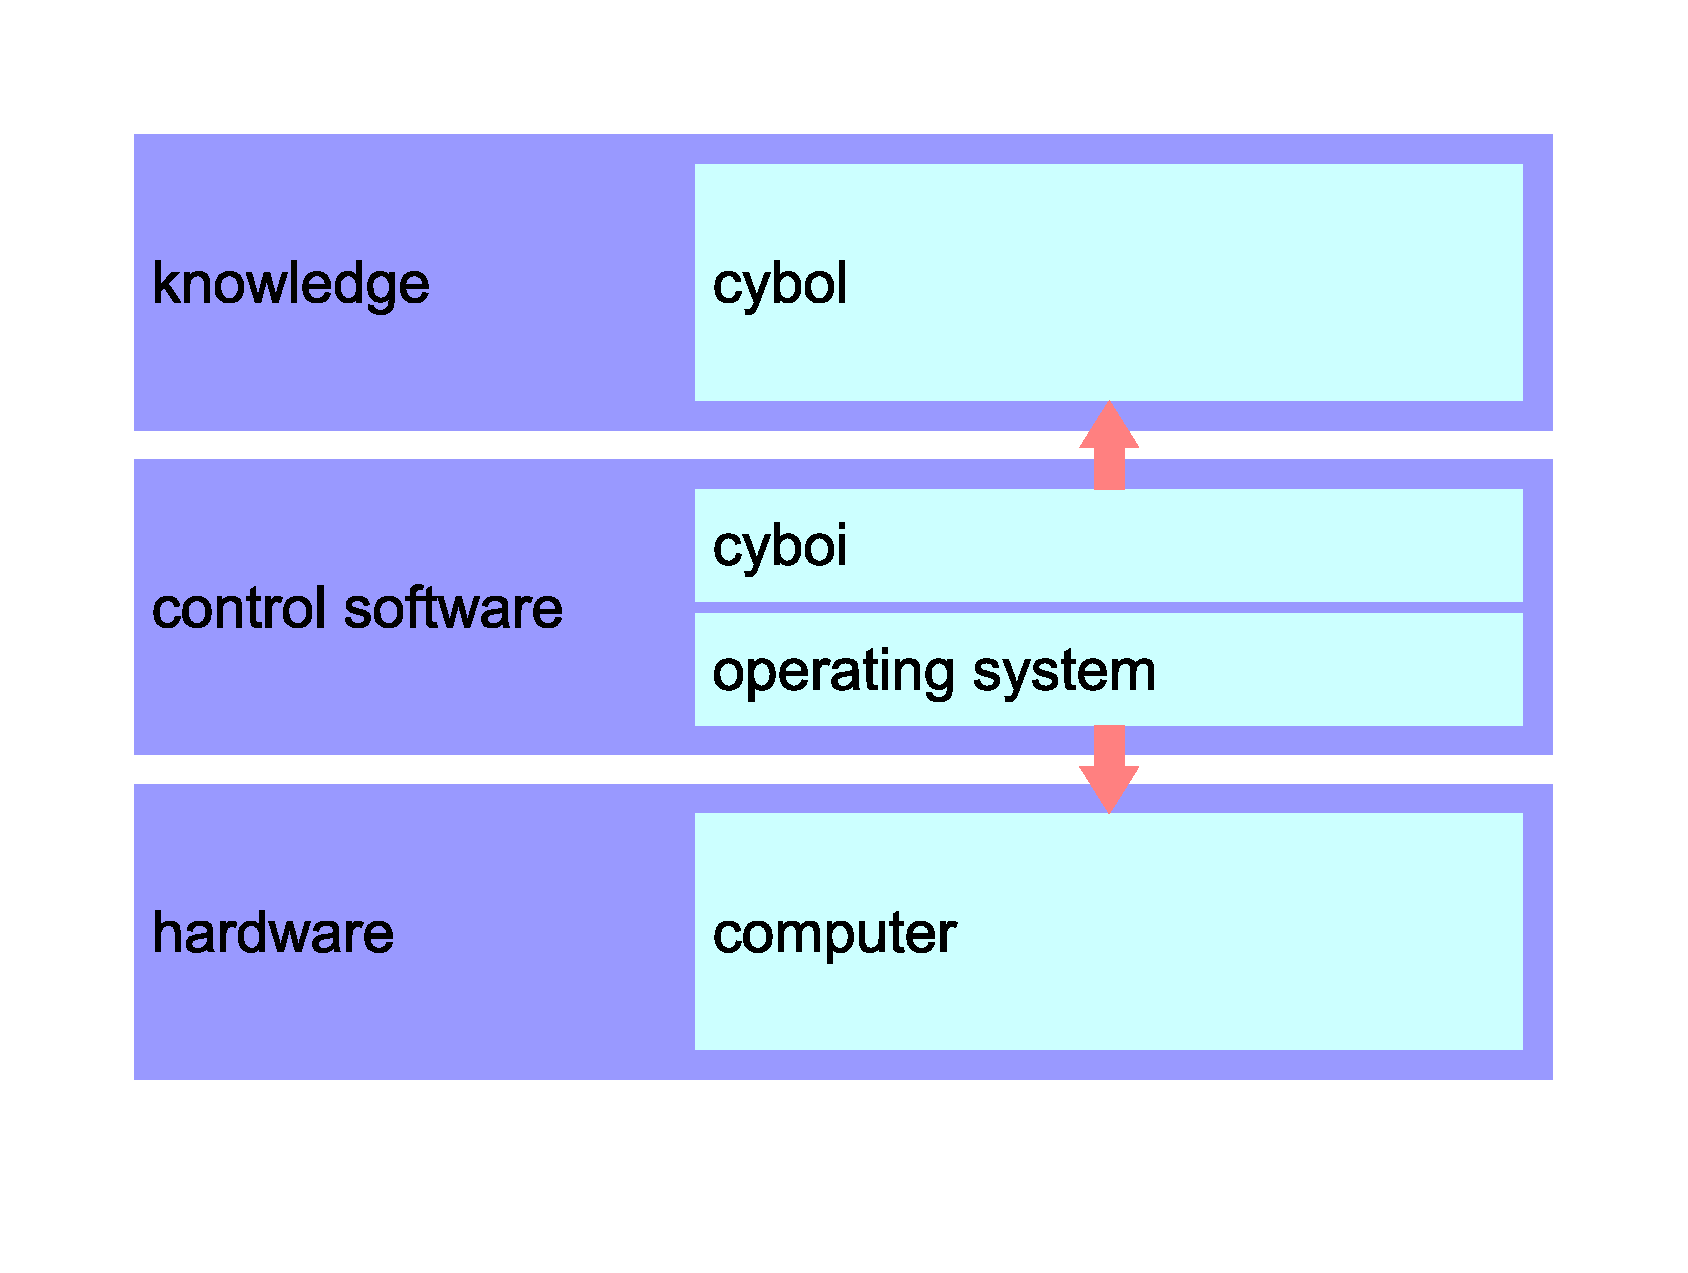
\includegraphics[scale=0.2]{vector/connection.eps}
        \caption{Knowledge -- Hardware Link}
        \label{connection_figure}
    \end{center}
\end{figure}

\begin{table}[ht]
    \begin{center}
        \begin{footnotesize}
        \begin{tabular}{| p{18mm} | p{18mm} | p{18mm} |}
            \hline
            \textbf{Criterion} & \textbf{Java World} & \textbf{CYBOP World}\\
            \hline
            Theory & OOP in Java & CYBOP\\
            \hline
            Language & Java & CYBOL\\
            \hline
            Interpreter & Java VM & CYBOI\\
            \hline
        \end{tabular}
        \end{footnotesize}
        \caption{Java-/ CYBOP World Analogies}
        \label{analogies_table}
    \end{center}
\end{table}

There are analogies to other systems run by language interpretation. Table
\ref{analogies_table} shows those between the \emph{Java-} and \emph{CYBOP}
world. Both are based on a programming theory, have a language and interpreter.
A theoretical model of a computer hardware- or -software system may be called
an \emph{Abstract Computer} or \emph{Abstract Machine} \cite{wikipedia}. If
being implemented as software simulation, or if containing an interpreter, it
is called a \emph{Virtual Machine} (VM). Kernighan and Pike write in their book
\emph{Practice of Programming} \cite{kernighan1999}:

\begin{quote}
� � Virtual machines are a wonderful, old idea, that latterly, through Java and
    the \emph{Java Virtual Machine} (JVM), came into fashion again. They are a
    simple possibility to gain portable and efficient program code, which can
    be written in a higher programming language.
\end{quote}

In that sense, CYBOI is certainly a VM. It provides low-level, platform-dependent
system functionality, close to the OS, together with a unified knowledge schema
(section \ref{knowledge_schema_heading}) which allows CYBOL applications to be
truly portable, well extensible and easier to program, because developers need
to concentrate on domain knowledge only. Since CYBOI interprets CYBOL sources
\emph{live} at system runtime, without the need for previous compilation (as in
Java), changes to CYBOL sources get into effect right away, without restarting
the system.

%
% $RCSfile$
%
% Copyright (c) 2005-2006. Christian Heller. All rights reserved.
%
% Permission is granted to copy, distribute and/or modify this document
% under the terms of the GNU Free Documentation License, Version 1.1 or
% any later version published by the Free Software Foundation; with no
% Invariant Sections, with no Front-Cover Texts and with no Back-Cover
% Texts. A copy of the license is included in the section entitled
% "GNU Free Documentation License".
%
% http://www.cybop.net
% - Cybernetics Oriented Programming -
%
% http://www.resmedicinae.org
% - Information in Medicine -
%
% Version: $Revision$ $Date$ $Author$
% Authors: Christian Heller <christian.heller@tuxtax.de>
%

\subsubsection{Architecture}
\label{architecture_heading}

To what concerns its inner architecture, there are two basic structures
underlying CYBOI:

\begin{enumerate}
    \item \emph{Knowledge Container:} An array-based structure usable for
        storing static knowledge in form of primitive- and compound models, and
        capable of representing a map, collection, list and tree
    \item \emph{Signal Checker:} A loop-based structure usable for dynamically
        reading signals from a queue, and capable of processing them after
        their priority, in a special handler
\end{enumerate}

\begin{figure}[ht]
    \begin{center}
        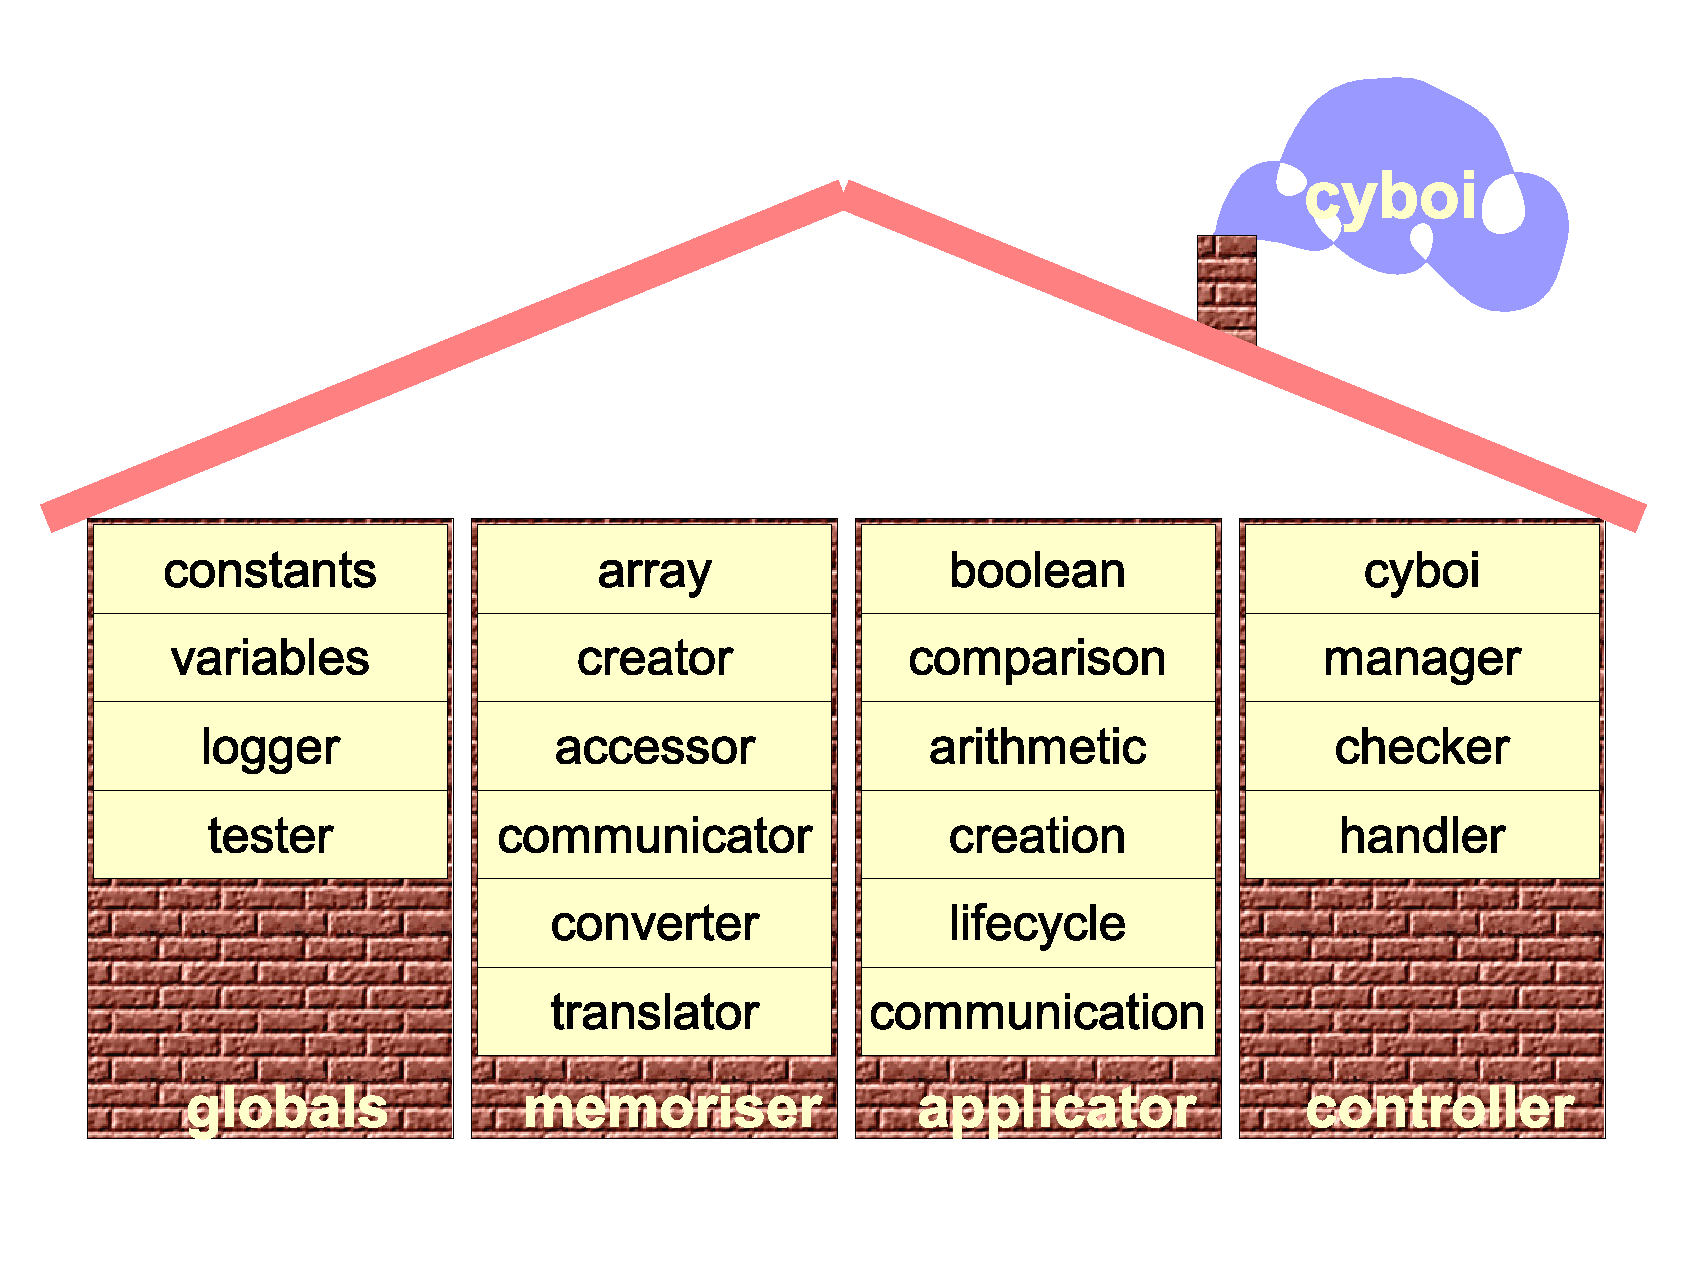
\includegraphics[scale=0.2]{vector/architecture.eps}
        \caption{CYBOI Architecture}
        \label{architecture_figure}
    \end{center}
\end{figure}

All modules, into which CYBOI is subdivided, are built around these two core
structures. Not unlike John von Neumann's model of a computing machine
\cite{selflinux}, which distinguishes \emph{Memory}, \emph{Control Unit},
\emph{Algorithmic Logic Unit} (ALU) and \emph{Input/ Output} (i/o), CYBOI's
modules are grouped into four architectural parts, as illustrated in figure
\ref{architecture_figure}. These have the following functionality:

\begin{itemize}
    \item \emph{Memoriser:} data creation, -destruction and -access (after
        Neumann, it contains not only data, but also the operations that are
        applied to them)
    \item \emph{Controller:} lifecycle management, signal handling, i/o filters
    \item \emph{Applicator:} operation application (comparison, logic,
        arithmetic and more)
    \item \emph{Globals:} basic constants and variables, as well as a logger
\end{itemize}

The i/o data handling is not separated out here (as opposed to von Neumann's
model); it is managed by the controller modules. The i/o data themselves,
representing states, are stored in memory.

%
% $RCSfile$
%
% Copyright (c) 2005-2006. Christian Heller. All rights reserved.
%
% Permission is granted to copy, distribute and/or modify this document
% under the terms of the GNU Free Documentation License, Version 1.1 or
% any later version published by the Free Software Foundation; with no
% Invariant Sections, with no Front-Cover Texts and with no Back-Cover
% Texts. A copy of the license is included in the section entitled
% "GNU Free Documentation License".
%
% http://www.cybop.net
% - Cybernetics Oriented Programming -
%
% http://www.resmedicinae.org
% - Information in Medicine -
%
% Version: $Revision$ $Date$ $Author$
% Authors: Christian Heller <christian.heller@tuxtax.de>
%

\subsubsection{Functionality}
\label{functionality_heading}

Figure \ref{cyboi_figure} shows three main parts of CYBOI. (The \emph{Globals}
package is neglectable for the following explanations, since it contains static
constants and variables that are \emph{omnipresent}.) The \emph{Controller}
manages system startup, shutdown and the handling of signals during its
runtime; the system uses just one central signal checking loop. The
\emph{Memoriser} provides memory structures (to store knowledge) and procedures
to access these. Logic knowledge is processed in the \emph{Applicator}.

\begin{figure}[ht]
    \begin{center}
        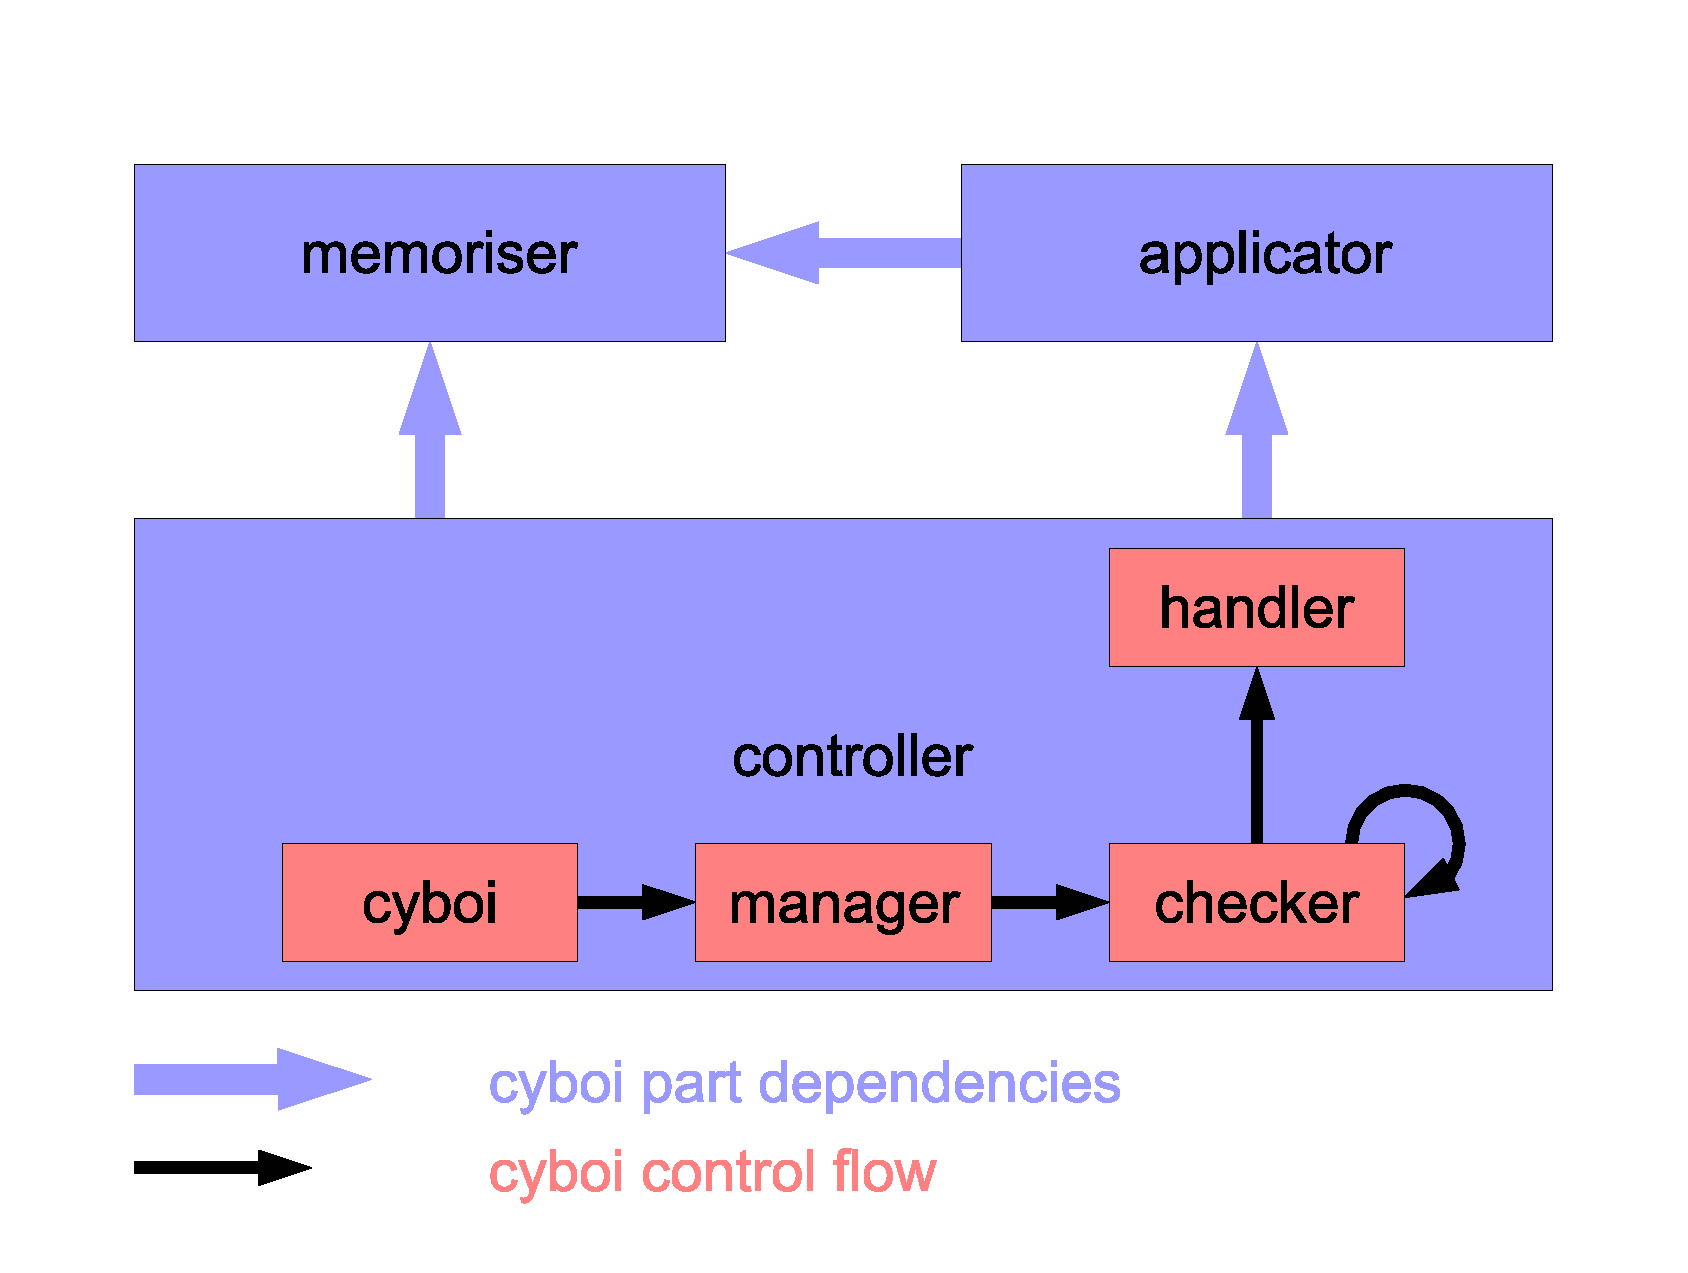
\includegraphics[scale=0.2]{vector/dependencies.eps}
        \caption{Dependencies and Control Flow}
        \label{cyboi_figure}
    \end{center}
\end{figure}

